\subsection{Architektura}
Projekt został zrealizowany w oparciu o wzorzec projektowy \textbf{MVVM} (Model-View-ViewModel), który został odpowiednio dostosowany do specyfiki aplikacji w celu zapewnienia modularności oraz uproszczenia procesu modyfikacji i rozbudowy.

\textbf{Adaptacja wzorca MVVM}
\begin{figure}[h!]
    \centering
    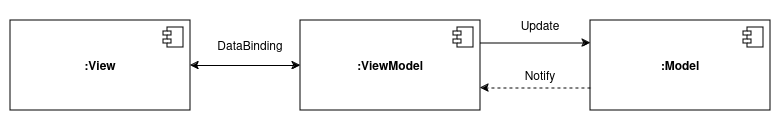
\includegraphics[width=0.8\textwidth]{img/diagramy/architektura.png}
    \caption{Schemat zaadaptowanego wzorca MVVM w projekcie.}
\end{figure}

W zaimplementowanym rozwiązaniu wzorzec \textbf{MVVM} został zmodyfikowany w celu optymalizacji komunikacji między komponentami aplikacji. Dzięki temu możliwe było osiągnięcie spójności architektury oraz jej wysokiej skalowalności.

\subsubsection{Opis komponentów architektury}
\begin{figure}[h!]
    \centering
    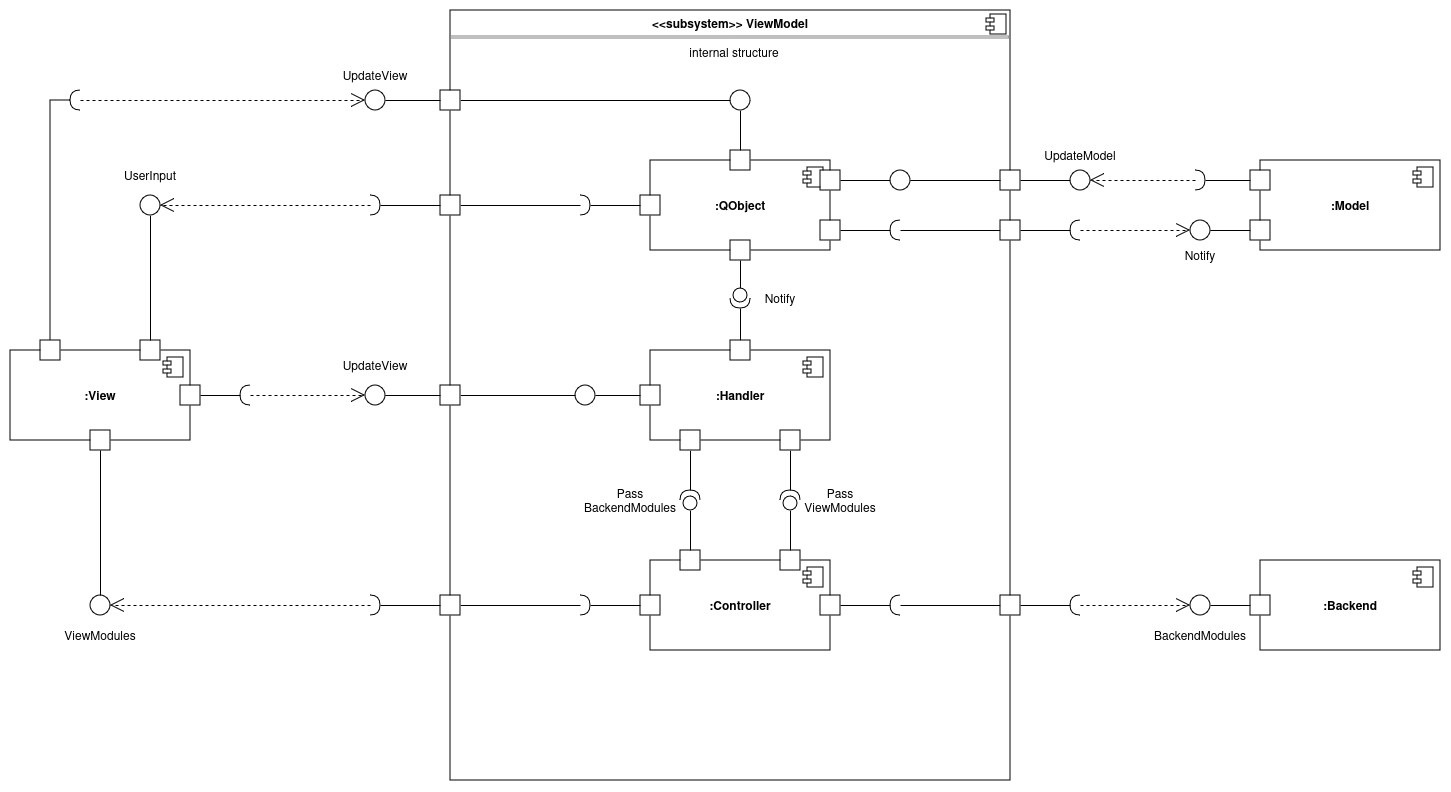
\includegraphics[width=0.8\textwidth]{img/diagramy/diagram_komp_vm.png}
    \caption{Struktura komponentów ViewModel w projekcie.}
\end{figure}

\textbf{ViewModel jako centralny element}
W projekcie klasa \texttt{ViewModel} zastępuje tradycyjny zbiór klas, takich jak:
\begin{itemize}
    \item \texttt{Controller} -- odpowiadający za sterowanie logiką,
    \item \texttt{QObject} -- obsługujący komunikację z frontendem,
    \item \texttt{Handler} -- integrujący dodatkowe funkcjonalności wizualne.
\end{itemize}

\textbf{Rola \texttt{QObject}}
Klasa \texttt{QObject} pełni funkcję tradycyjnego komponentu \texttt{ViewModel}, umożliwiając komunikację między warstwą logiki a frontendem aplikacji. Wykorzystuje mechanizm sygnałów dostarczany przez bibliotekę PyQt, co pozwala dynamicznie informować widok o zmianach stanu aplikacji.

\textbf{Handler jako rozszerzenie funkcjonalności}
\texttt{QObject} został wzbogacony o klasę \texttt{Handler}, która pozwala na łatwą implementację funkcji wizualnych w już istniejącej architekturze. Dzięki temu projekt zachowuje przejrzystość i elastyczność.

\textbf{Integracja za pomocą \texttt{Controller}}
Klasy \texttt{QObject} i \texttt{Handler} są zintegrowane za pomocą \texttt{Controller}, który zapewnia jednolity interfejs oraz ułatwia zarządzanie komponentami aplikacji.

Na diagramie widoczny jest dodatkowy komponent \textbf{Backend}, będący zbiorem skryptów, które dostarczają interfejs dla wymaganej funkcjonalności aplikacji. Backend odpowiada za obsługę logiki niezwiązanej bezpośrednio z widokiem oraz wspiera pozostałe komponenty architektury, zapewniając większą modularność.

\subsubsection{Zalety wdrożonego rozwiązania}
Przedstawione rozwiązanie zapewnia następujące korzyści:
\begin{itemize}
    \item \textbf{Modularność} -- możliwość łatwego dodawania i modyfikowania komponentów bez ingerencji w istniejącą strukturę.
    \item \textbf{Skalowalność} -- umożliwia rozbudowę aplikacji o nowe funkcjonalności przy zachowaniu spójności architektury.
    \item \textbf{Wsparcie dla współbieżności} -- dzięki zastosowaniu mechanizmu sygnałów PyQt implementacja współbieżności jest intuicyjna i efektywna.
\end{itemize}

\subsubsection{Podsumowanie}
Zaimplementowany wzorzec MVVM, w połączeniu z dodatkowymi modyfikacjami, pozwolił osiągnąć elastyczną i skalowalną architekturę aplikacji. Dzięki zastosowanemu podejściu projekt spełnia założenia modularności, umożliwiając łatwą rozbudowę oraz utrzymanie w przyszłości.

\end{document}